\documentclass[pdf,aspectratio=169]{beamer}
\usepackage[]{hyperref,graphicx,siunitx,lmodern,booktabs}
\usepackage{physics}
\usepackage{em-commands}
\mode<presentation>{\usetheme{EM}}

%Question Numbering
\newcounter{questionnumber}
\newcommand{\qnum}{%
	\stepcounter{questionnumber}%
	Q\arabic{questionnumber}
}
\resetcounteronoverlays{questionnumber}

\graphicspath{ {../Images/} }

\sisetup{per-mode=symbol}

%preamble
\title{Reflections of the Real World}
\date{September 26, 2018}
\author{Jed Rembold}

\begin{document}
\renewcommand{\theenumi}{\Alph{enumi}}

\begin{frame}{Announcements}
	\begin{itemize}
		\item Homework 5 posted!
			\begin{itemize}
				\item Only 4 problems this time, and 1 is really easy
				\item Two are quite computer heavy though
				\item Lots of plotting throughout
			\end{itemize}
		\item Start reading Ch 3.3, but we won't talk about Separation of Variables until Monday probably
		\item Bring your laptop on Friday, as we'll probably try to use them
	\end{itemize}
\end{frame}

\begin{frame}{\qnum}
	You and I are solving two entirely different problems, both of which have no charge density in our region of interest. What can you deduce about our two solutions?
	\begin{enumerate}
		\item Our solutions will be the same, due to uniqueness
		\item \alert<2>{Our solutions will be the same if we also have the same boundary conditions}
		\item Our solutions will be the same if we also our boundary conditions are both continuous
		\item Our solutions will be the same if our regions of interest intersect
	\end{enumerate}
\end{frame}

\begin{frame}{\qnum}
	Can a grounded conductor ($V=0$) have a surface charge density on it?
	\begin{enumerate}
		\item \alert<2>{Yes}
		\item No
		\item Only if it has cavities inside it
	\end{enumerate}
\end{frame}

\begin{frame}{\qnum}
	\begin{columns}
		\column{0.5\textwidth}
		Solving the problem to the right with two charges above a grounded plane is akin to solving which of the below configurations?
		\column{0.4\textwidth}
		\begin{center}
			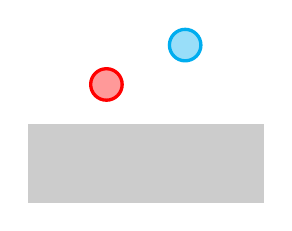
\begin{tikzpicture}
				\fill[gray!40] (0,0) rectangle +(3,1);
				\draw[very thick, Red, fill=red!40] (1,1.5) circle (2mm);
				\draw[very thick, cyan, fill=cyan!40] (2,2) circle (2mm);
			\end{tikzpicture}
		\end{center}
	\end{columns}
	\begin{center}
		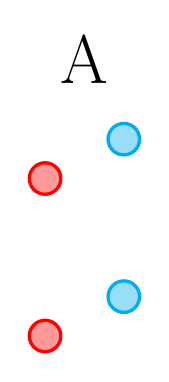
\begin{tikzpicture}
			\node[font=\Huge] at (1.5,3) {A};
			\draw[very thick, Red, fill=red!40] (1,1.5) circle (2mm);
			\draw[very thick, cyan, fill=cyan!40] (2,2) circle (2mm);
			\draw[very thick, Red, fill=red!40] (1,-0.5) circle (2mm);
			\draw[very thick, cyan, fill=cyan!40] (2,0) circle (2mm);
		\end{tikzpicture}\hspace{2cm}
		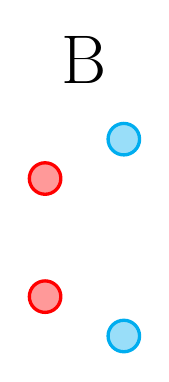
\begin{tikzpicture}
			\node[font=\Huge] at (1.5,3) {B};
			\draw[very thick, Red, fill=red!40] (1,1.5) circle (2mm);
			\draw[very thick, cyan, fill=cyan!40] (2,2) circle (2mm);
			\draw[very thick, Red, fill=red!40] (1,0) circle (2mm);
			\draw[very thick, cyan, fill=cyan!40] (2,-0.5) circle (2mm);
		\end{tikzpicture}\hspace{2cm}
		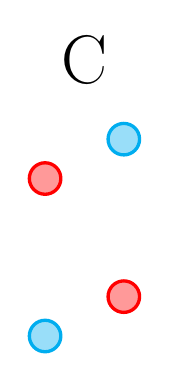
\begin{tikzpicture}
			\node[font=\Huge] at (1.5,3) {C};
			\draw[very thick, Red, fill=red!40] (1,1.5) circle (2mm);
			\draw[very thick, cyan, fill=cyan!40] (2,2) circle (2mm);
			\draw[very thick, Red, fill=red!40] (2,0) circle (2mm);
			\draw[very thick, cyan, fill=cyan!40] (1,-0.5) circle (2mm);
		\end{tikzpicture}\hspace{2cm}
		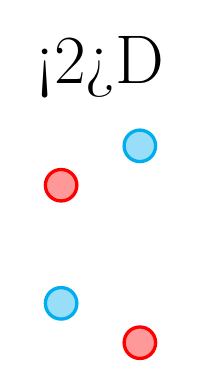
\begin{tikzpicture}
			\node[font=\Huge] at (1.5,3) {\alert<2>{D}};
			\draw[very thick, Red, fill=red!40] (1,1.5) circle (2mm);
			\draw[very thick, cyan, fill=cyan!40] (2,2) circle (2mm);
			\draw[very thick, Red, fill=red!40] (2,-0.5) circle (2mm);
			\draw[very thick, cyan, fill=cyan!40] (1,0) circle (2mm);
		\end{tikzpicture}
	\end{center}
\end{frame}

\begin{frame}{\qnum}
	Can you use the method of images to solve situations with multiple grounded planes? Say you had a charge living beside two conducting planes.
	\begin{columns}
		\column{0.5\textwidth}
		\begin{center}
			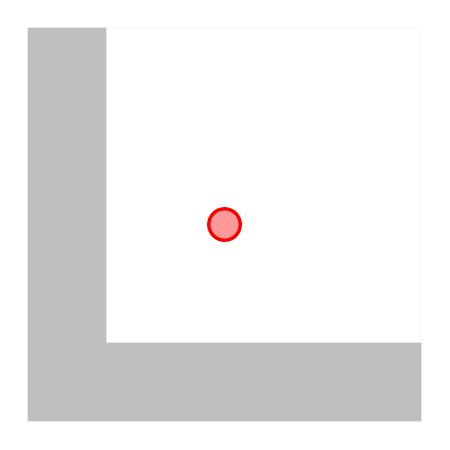
\begin{tikzpicture}
				\fill[gray!50, even odd rule] (0,0) rectangle (5,5) (1,1) rectangle (5,5);
				\draw[very thick, Red, fill=red!40] (2.5, 2.5) circle (2mm);
			\end{tikzpicture}
		\end{center}
		
		\column{0.5\textwidth}
		\begin{enumerate}
			\item Yes, and it would take 3 charges
			\item \alert<2>{Yes, and it would take 4 charges}
			\item No, it would take an infinite number of charges
			\item No, you can not combine conducting planes with the method of images
		\end{enumerate}
	\end{columns}
\end{frame}

\begin{frame}{\qnum}
	What if instead the grounded planes were at an angle to one another. Could you still use the method of images?
	\begin{columns}
		\column{0.4\textwidth}
		\begin{enumerate}
			\item Yes
			\item No
			\item \alert<2>{Sometimes?}
		\end{enumerate}
		\column{0.5\textwidth}
		\begin{center}
			\begin{tikzpicture}
				\draw[line width=8pt, gray!50] (0,0) -- +(45:4) (0,0) -- +(0:4);
				\draw[very thick, Red, fill=red!40] (3,1) circle (2mm);
				\draw[<->, thick] (1,0) arc (0:45:1cm) node[midway,right,math] {\theta};
			\end{tikzpicture}
		\end{center}
	\end{columns}
\end{frame}

\begin{frame}{\qnum}
	Could you use the method of images if the grounded planes formed a kind of Death Star trench around the charge?
	\begin{columns}
		\column{0.5\textwidth}
		\begin{center}
			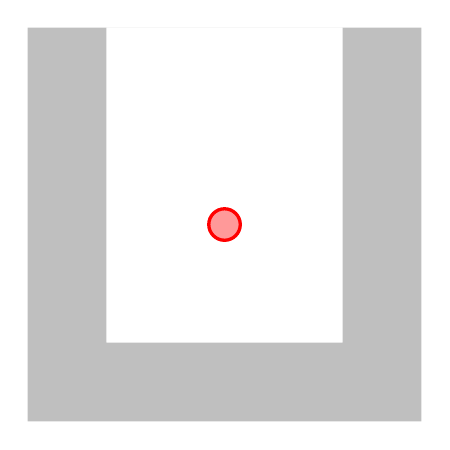
\begin{tikzpicture}
				\fill[gray!50, even odd rule] (0,0) rectangle +(5,5) (1,1) rectangle (4,5);
				\draw[very thick, Red, fill=red!40] (2.5,2.5) circle (2mm);
			\end{tikzpicture}
		\end{center}
		
		\column{0.5\textwidth}
		\begin{enumerate}
			\item Yes, it would take 4 total charges
			\item Yes, it would take 6 total charges
			\item Yes, it would take 9 total charges
			\item \alert<2>{No, method of images will not work here}
		\end{enumerate}
	\end{columns}
\end{frame}

\begin{frame}{\qnum}
	Like potential, energy is the same between configurations when using the method of images.
	\begin{enumerate}
		\item True
		\item \alert<2>{False}
	\end{enumerate}
\end{frame}




\end{document}
